%!TEX root = ../report.tex
\chapter{Experimental Setup}

%How you are planning to test/compare/evaluate your research.
%Criteria used.
\section{Dataset}

Mohler et al (2009)\cite{Mohler2009} consists of questions from Introductory comuter science assignments along with answers given by undergraduate students. The assignments were monitored by the University of North Texas. The dataset consists of 3 assignments, each assignment consists of 7 short answer questions and each question has answers given by 30 students. Overall dataset consists of 630 students answers, their grades randing from 0 to 5, and the model answers written by the instructors. 

Mohler et al (2011)\cite{Mohler2011} created a dataset from the data structure course University of North Texas and the dataset consist of 2273 answers written by 31 students for 80 questions. The grades for this 2273 answers were given by two human expert graders in that particular domain.

\section{Data Preprocessing}

Each of the answer in the dataset were processed using various NLP preprocessing techniques. These methods are as listed below;

\begin{itemize}
	\item Normalization - The answers were converted into lowercase so that all the text are in equal footing. Following that, the punctuations in the answers were removed using a regular expression function. 
	\item Stop words removal - The most common occuring words such as 'the', 'it' etc. were removed from the student answers. NLTK corpus's stop words dictionary was used for this task.
	\item Lemmatization - Each and every word in the student's answers were converted into their common form / root form and the resulting text were used in the feature extraction stage. Textblob's lemmatize function, which is learned based on the WordNet's lexical database, was used for this task. 
\end{itemize}

\section{Features Used}

The answers which are preprocessed as discussed in the above section were used to extract features in this stage. In this experiment, a simple feature extraction method called Bag-of-words approach was used. Each word in the students' answers is tokenized and every token is counted based on the number of occurrences. Scikit-learn's feature extraction method called 'CountVectorizer' was used for this task which produces a sparse representation of the count of each words as a matrix.

\subsection{Interface}

A Javascipt based web interface was used to display the process of querying the labels from a human expert / professor. Vue.js was used in the backend for the dynamic nature of display (changing the question and answer being displayed at a time). The interface consists of Fields for question, answer, grade predicted by the model, professor's grade, positive feedback and negative feedback. A screenshot of the interface used in this experiment is shown in Fig.\ref{gui_layout}.

\begin{figure}[h]
	\centering
	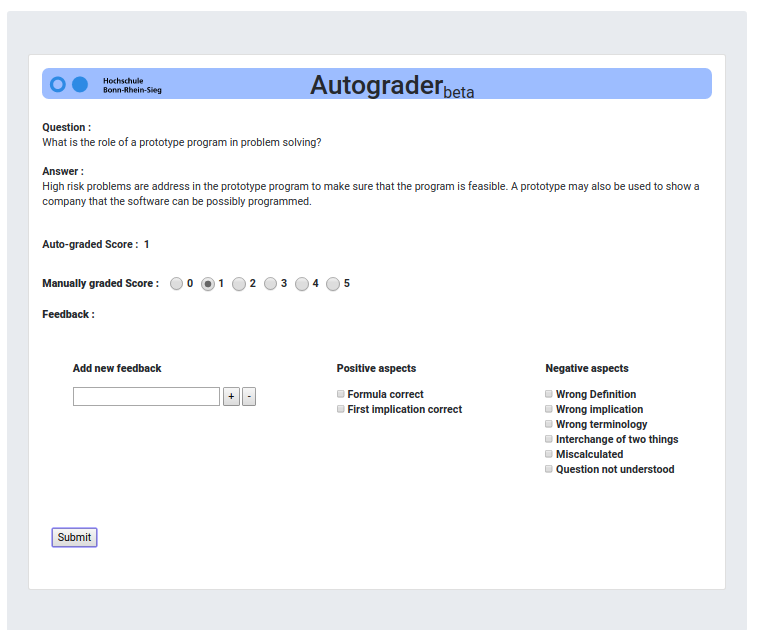
\includegraphics[scale=0.6]{images/gui_layout}
	\caption{Interface used in the experiment for the querying purpose}
	\label{gui_layout}
\end{figure}

\section{Experimental Setup}

\subsection{Experiment 1}

The experiments were conducted on the datasets discussed above. A Graphical User Interface was designed to label the queried instance (correct grades for each answer) by the professor. The details of this GUI would be discussed in the Interface section below. 

The raw questions and answers from the dataset were preprocessed using various NLP techniques and the required features were extracted from them to learn a model. The model would be learned initially from a few labeled instances (graded answers) and then it learns from newly labeled answers using a machine learning paradigm called Active Learning. The experimental pipeline of the experiment is shown in the figure below.

\begin{figure}[h]
	\centering
	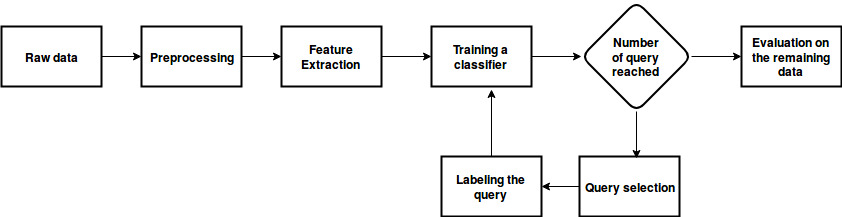
\includegraphics[scale=0.5]{images/exp_design}
	\caption{The basic pipeline of our experimental design}
	\label{exp_pipeline}
\end{figure}

\subsubsection{Algorithm and Methodology}

Once the dataset is cleaned and preprocessed as discussed above, Scikit-learn's Logistic regression classifier was used to classify the answers based on the features extracted. Two tasks were performed using this model. 

\begin{itemize}
	\item Binary classification - The answers which had more than 3 and up to 5 marks were considered as a positive class (1) and the ones which had less than 3 were considered the negative class (0). 
	
	\item Multi-class classification - The grades of each answer was rounded off to a whole number between 0 to 5 and a classifier is trained to predict the correct class for each of them in these five classes. 
\end{itemize}

The classifier was initially trained on one answer per each class and the labels / grades for the next answer for the model to learn on was selected using the Pool-based uncertainty sampling strategy discussed above in the Active Learning section. The best answer to be queried next is selected based on how uncertain / confused the algorithm is about the different classes it can take.  The algorithm shown in the Fig. \ref{uncertainty-al} below explains this process. 

\begin{figure}[h]
	\centering
	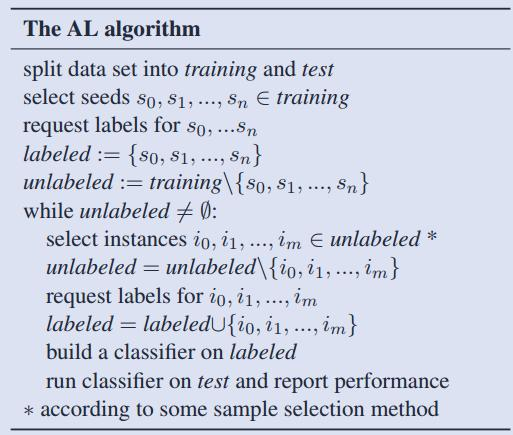
\includegraphics[scale=0.6]{images/uncertainty-al-pseudocode}
	\caption{Pseudocode for general, pool-based active learning. \cite{Horbach2016}.}
	\label{uncertainty-al}
\end{figure}

In our experiments, the number of instances to query from the human expert was set to 40. This is only about 7\% of the Mohler et al. 2009 dataset and just 1.6\% of the Mohler et al. 2011 dataset. 


\subsection{Experiment 2}

In this experimental setup, users were asked to use the interface with and without the influence of active learning on just 40 answers and were asked to give feedbacks on their user experience.  

The raw questions and answers from the dataset were preprocessed using various NLP techniques as discussed above and the required features were extracted from them to learn a model. The model would be learned initially from a few labeled instances (graded answers) and then it learns from newly labeled answers using a machine learning paradigm called Active Learning.

\subsubsection{Algorithm and Methodology}

Once the dataset is cleaned and preprocessed as discussed above, Scikit-learn's Logistic regression classifier was used to classify the answers based on the features extracted. Two tasks were performed using this model. 

\begin{itemize}
	\item Without active learning - In the non-active learning phase, the questions and answers were displayed to the user one by one, without any indication of the correct answer. The users had to decide between two grades (0 for a wrong answer and 1 for a correct answer). This setup reflects the usual way of grading answers. 
	
	\item With active learning - In the phase with active learning, the answers predicted by the active learning model (which was trained with five queries) was displayed to the user. The predictions were set in the radio button for each answer so that given the correct prediction, the user doesn't have to just submit it and move on to the next question, thus reducing the effort and time of clicking the right grade. 
\end{itemize}

The classifier was initially trained on one answer per each class and the labels / grades for the next answer for the model to learn on was selected using the Pool-based uncertainty sampling strategy discussed above in the Active Learning section. The best answer to be queried next is selected based on how uncertain / confused the algorithm is about the different classes it can take. 

%\section{Experimental Design}
